\subsection*{Acquisition and Synchronization}
\textbf{Carrier Recovery:}

We want to cancel phase error. This in turn cancel
the frequency error as frequency is phase speed. We use a PLL (Phase Locked Loop)
to do so. The PLL is a feedback loop that compares the phase of the received signal
with the phase of the local oscillator. The phase error is then used to correct
the local oscillator phase.

\setlength{\intextsep}{-10pt}
\begin{wrapfigure}{r}{0.3\columnwidth}
    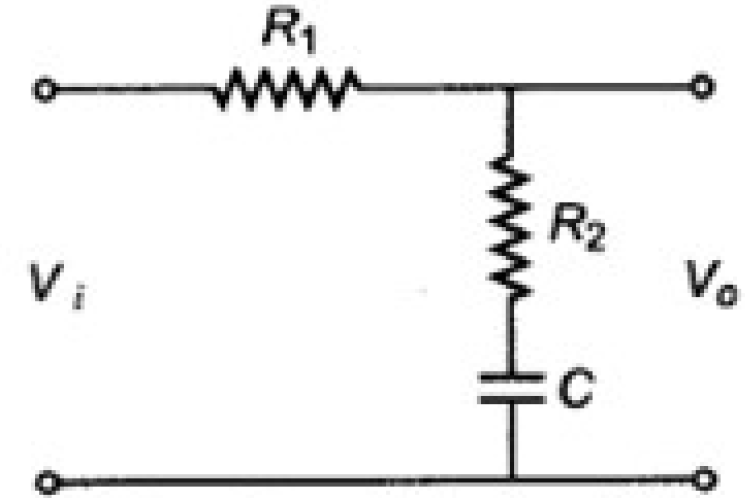
\includegraphics[width=\linewidth]{images/pll_loop_filter.png}
\end{wrapfigure}
\underline{Transfert function of the PLL:}

$H(s)=\frac{\frac{KG(s)}{s}}{1+\frac{KG(s)}{s}}$

where $G(s)=\frac{1+\tau_2s}{1+\tau_1s}$

with $\tau_1=C(R_1+R_2)$ and $\tau_2=C(R_2)$.

$\omega_n=\sqrt{\sfrac{K}{\tau_1}}$,

$\zeta=\frac{\omega_n(\tau_2+\sfrac{1}{K})}{2}$

Acquisition performance of the loop is the characteristics when it goes from unlocked state to
complete phase lock. Tracking behavior is the ability of the loop to follow variations at the
input.

\textbf{Symbol synchronizer:}

There are several ways to extract a clock from a data stream.
We can classify them in two categories:

\underline{Decision directed:}

We try to take samples without
exact timing and then take a decision with a
maximum likelihood criteria.


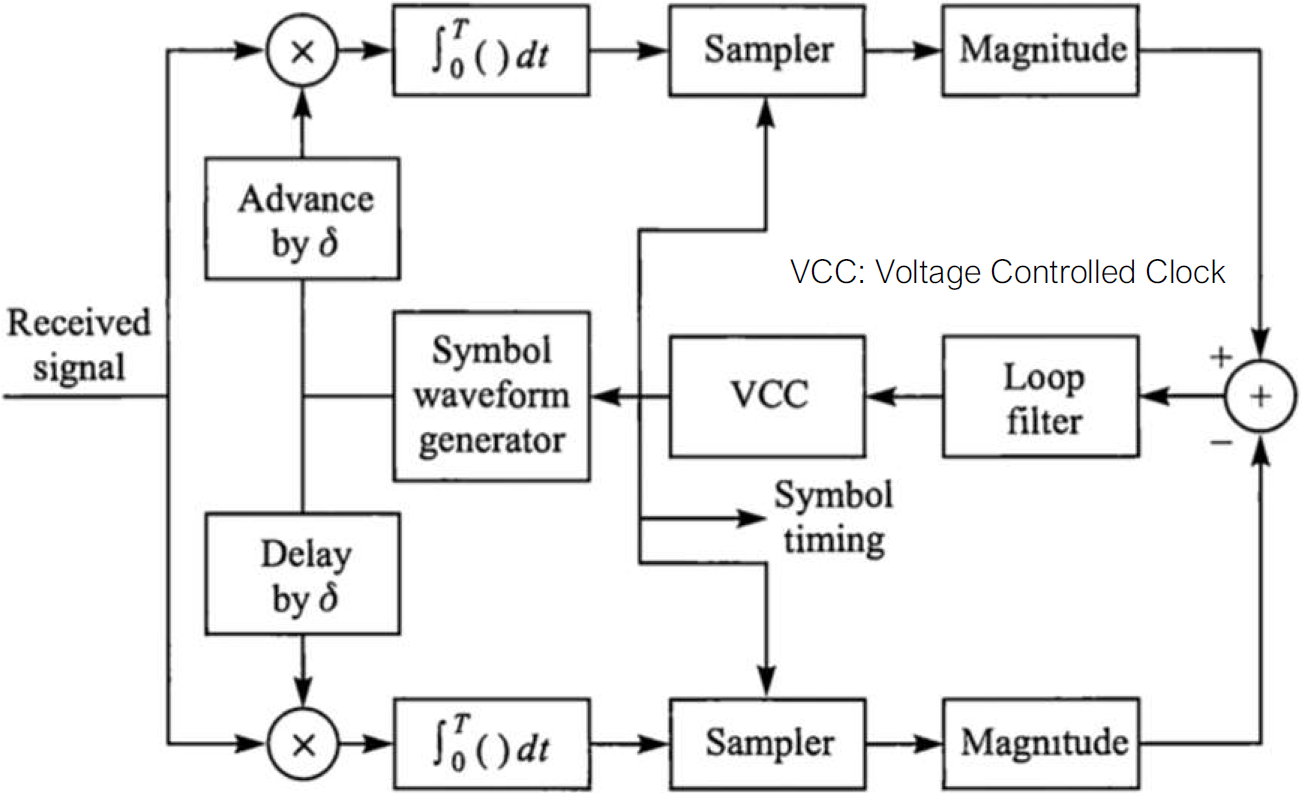
\includegraphics[width=\columnwidth]{images/early_state_synch.png}

\underline{Non decision directed:}

Geting a maximum likelihood on the symbol shape. For example
with a

\underline{Early-late synchronizer}:

We can create a system where we compute the difference between the correlation with shift
$+\delta$ and $-\delta$. If the difference is null we have the optimum otherwise we shift.

The channel can be represented by its transfer function. Equalization is the estimation and application of this
transfer function. This allows to fight ISI. But with OFDM we have long guard intervals that
render equalization unnecessary.